% arara : pdflatex
% arara : bibtex
% arara : pdflatex
% arara : pdflatex

\documentclass[a4paper]{article}
\usepackage[T1]{fontenc}
\usepackage[italian]{babel}

\usepackage{enumitem}   % Gestisce le liste numerata
\setlist[enumerate,1]{label=\arabic* )} 
\usepackage{amsmath}    % Usato pe la matematica
\usepackage{booktabs}   % Gestisce le tabelle
\usepackage{tikz-cd}    % Usato per creare grafiche
\usepackage{numprint}   % Usato per stampare i numeri con sepatori alle migliaia
\usepackage{listings}   % Usato per avere un enviroment per il codice

\definecolor{codegray}{rgb}{0.5,0.5,0.5}
\definecolor{codepurple}{rgb}{0.58,0,0.82}
\definecolor{backcolour}{rgb}{0.95,0.95,0.92}
\lstdefinestyle{mystyle}{
    backgroundcolor=\color{backcolour},   
    keywordstyle=\color{blue},
    numberstyle=\tiny\color{codegray},
    stringstyle=\color{codepurple},
    basicstyle=\ttfamily\footnotesize,
    numbers=left,    
    breaklines=true,                
    numbersep=-10pt,                  
    tabsize=2
}
\lstset{style=mystyle}

% \usepackage{showkeys}   % Usato per vedere le label
% \usepackage{showframe}  % Usato per vedere i frame

\newtheorem{theorem}{Teorema}[section]

\newcommand{\code}[1]{
    \texttt{#1}
}

\begin{document}

\title{Parallelizzazione dell'algoritmo di intersezione di Möller\-Trumbore}
\author{Gallina Roberto}
\date{06/11/2023}

\maketitle

\newpage

\tableofcontents

\newpage

\section{Algoritmo di Möller\-Trumbore}
L'algoritmo di intersezione di Möller\-Trumbore è un metodo usato per capire se un raggio (linea con un punto d'inzio e una direzione) intersecano un triangolo nello spazio 3D.
è usato nella Computer Graphics per determinare quali parti di modelli 3D sono visibili da un certo punto di vista.

\begin{figure}[htp]
    \begin{lstlisting}[language=c++]
    bool RayIntersectsTriangle(
        Vector3D rayOrigin, 
        Vector3D rayVector, 
        Triangle* inTriangle,
        Vector3D& outIntersectionPoint
    ){
        const float EPSILON = 0.0000001;
        Vector3D vertex0 = inTriangle->vertex0;
        Vector3D vertex1 = inTriangle->vertex1;  
        Vector3D vertex2 = inTriangle->vertex2;
        
        Vector3D edge1, edge2, h, s, q;
        edge1 = vertex1 - vertex0;
        edge2 = vertex2 - vertex0;
        
        float a, f, u, v;
        h = rayVector.crossProduct(edge2);
        a = edge1.dotProduct(h);
        
        if (a > -EPSILON && a < EPSILON)
            return false;
        
        f = 1.0 / a;
        s = rayOrigin - vertex0;
        u = f * s.dotProduct(h);
        
        if (u < 0.0 || u > 1.0)
            return false;
            
        q = s.crossProduct(edge1);
        v = f * rayVector.dotProduct(q);
            
        if (v < 0.0 || u + v > 1.0)
            return false;
        
        float t = f * edge2.dotProduct(q);
        
        if (t > EPSILON){
            // ray intersection
            outIntersectionPoint = rayOrigin + rayVector * t;
            return true;
        }else
            return false;
    }
    \end{lstlisting}
    \caption{Algoritmo di Möller\-Trumbore da Wikipedia}
\end{figure}

\newpage

\section{Prima semplice implementazione}
Prima di procedere con la prima implementazione, va do a creare le strutture e le funzioni basilari che serviranno nei vari calcoli.

\subsection{Struttura Point3D}
\begin{lstlisting}[language=c++]
    struct Point3D{
        double x;
        double y;
        double z;
    };
\end{lstlisting}

\subsection{Struttura Triangle}
\begin{lstlisting}[language=c++]
    struct Triangle {
        Point3D p1;
        Point3D p2;
        Point3D p3;
    };

\end{lstlisting}

\subsection{Differenza tra vettori}
\begin{lstlisting}[language=c++]
    Point3D difference(Point3D a, Point3D b){
        return {a.x - b.x, a.y - b.y, a.z - b.z};
    }
\end{lstlisting}

\subsection{Dot product}
\begin{lstlisting}[language=c++]
    double dotProduct(Point3D &v1, Point3D &v2) {
        return v1.x * v2.x + v1.y * v2.y + v1.z * v2.z;
    }
\end{lstlisting}

\subsection{Cross product}
\begin{lstlisting}[language=c++]
    Point3D crossProduct(Point3D &v1, Point3D &v2) {
        return {
            v1.y * v2.z - v1.z * v2.y, 
            v1.z * v2.x - v1.x * v2.z,
            v1.x * v2.y - v1.y * v2.x
        };
    }
\end{lstlisting}

\newpage

\subsection{Codice}
Vado quindi ad implementare la versione del codice vista precedentemente

\begin{lstlisting}[language=c++]
    bool rayIntersectsTriangle(
        Point3D rayOrigin, 
        Point3D rayVector,
        Triangle inTriangle
    ){
        const float EPSILON = 0.0000001;
        Point3D vertex0 = inTriangle.p1;
        Point3D vertex1 = inTriangle.p2;
        Point3D vertex2 = inTriangle.p3;

        Point3D edge1, edge2, h, s, q;
        double a, f, u, v;

        edge1 = difference(vertex1, vertex0);
        edge2 = difference(vertex2, vertex0);

        h = crossProduct(rayVector, edge2);
        a = dotProduct(edge1, h);

        if (a > -EPSILON && a < EPSILON)
            return false;

        f = 1.0 / a;
        s = difference(rayOrigin, vertex0);
        u = f * dotProduct(s, h);

        if (u < 0.0 || u > 1.0)
            return false;

        q = crossProduct(s, edge1);
        v = f * dotProduct(rayVector, q);
        if (v < 0.0 || u + v > 1.0)
            return false;

        double t = f * dotProduct(edge2, q);

        if (t > EPSILON)
            return true;

        return false;
    }
\end{lstlisting}

\newpage

Implemento ora il `main` verificando che l'algoritmo funzioni correttamente sui casi base

\subsubsection{Raggio interseca triangolo}

\begin{lstlisting}[language=c++]
    int main() {
        Point3D rayOrigin = {0.0, 0.0, 0.0};
        Point3D rayDirection = {0.0, 0.0, 2.0};
        
        Triangle triangle = {
            {-0.5, 0.5, 0.5}, 
            {0.5, 0.0, 0.5}, 
            {0.5, -1.0, 0.5}
        };
        
        cout << rayIntersectsTriangle(rayOrigin, rayDirection, triangle);

        return 0;
    }
\end{lstlisting}

\begin{lstlisting}[language=bash,backgroundcolor=\color{black},basicstyle=\ttfamily\footnotesize\color{green}]
    1
\end{lstlisting}

\subsubsection{Raggio non interseca triangolo}

\begin{lstlisting}[language=c++]
    ..
    Triangle triangle = {
        {-0.5, 0.5, 0.5},
        {0.5, 0.5, 0.5},
        {0.5, -0.2, 0.5}
    };
    .. 
\end{lstlisting}

\begin{lstlisting}[language=bash,backgroundcolor=\color{black},basicstyle=\ttfamily\footnotesize\color{green}]
    0
\end{lstlisting}

\begin{figure}[ht]
    \centering
    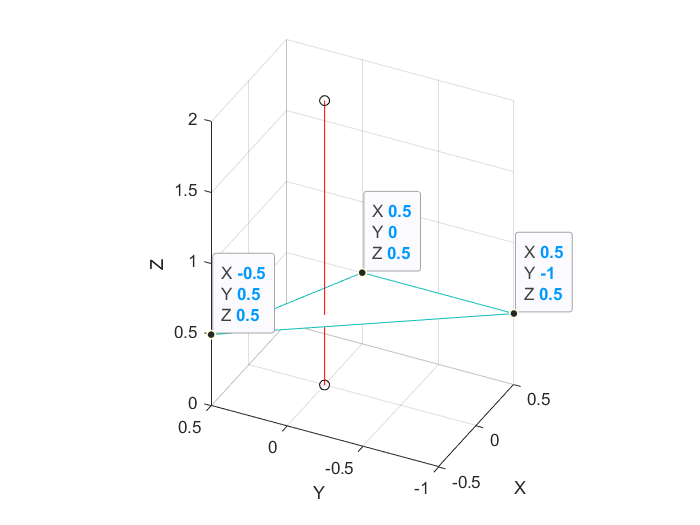
\includegraphics[width=0.48\textwidth]{images/intersect.png}
    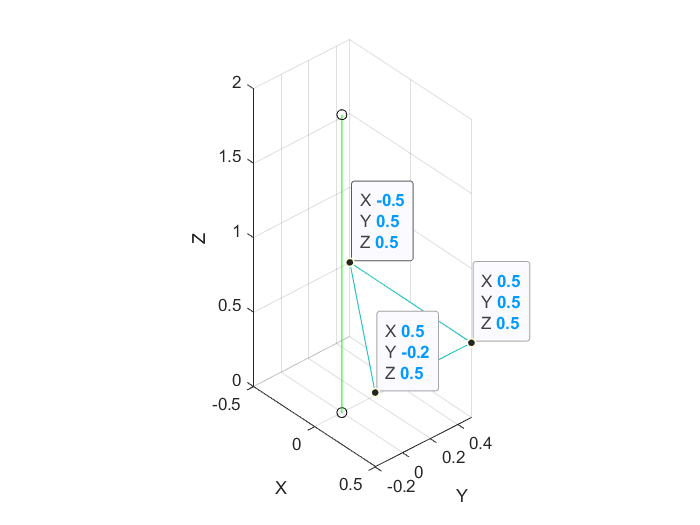
\includegraphics[width=0.48\textwidth]{images/notintersect.png}
\end{figure}

\newpage

\section{Esempio complesso}

\subsection{Lettura dei file}

Vado ora a implementare delle funzioni per poter leggere i file dei punti e delle mesh, sappiamo infatti che il file \emph{verts.csv} è composto da tre numeri con virgola scritti in notazione scentifica.

\vspace{5pt}

\noindent\emph{Es. \footnotesize{-6.195182353258132935e-02,-5.577753782272338867e-01,5.792263150215148926e-01}}

\vspace{7pt}

Vado quindi a creare una funzione che dato il nome del file genera un vettore di punti.

\begin{lstlisting}[language=c++]
    vector<Point3D> readPoints(string filename) {
        vector<Point3D> punti;
        string linea;
        ifstream file(filename);
        if (file.is_open()) {
            while (getline(file, linea)) {
                Point3D punto;
                stringstream ss(linea);
                string valore;
                if (getline(ss, valore, ',')) {
                    punto.x = stod(valore);
                }
                if (getline(ss, valore, ',')) {
                    punto.y = stod(valore);
                }
                if (getline(ss, valore)) {
                punto.z = stod(valore);
                }
                punti.push_back(punto);
            }
            file.close();
        }
        return punti;
    }
\end{lstlisting}

\newpage

Allo stesso modo sappiamo che il file \emph{mesh.csv} è composto da tre numeri scritti in notazione scentifica, corrispondenti al numero (indice) del punto.

\vspace{5pt}

\noindent\emph{Es. \footnotesize{1.000000000000000000e+00,2.000000000000000000e+00,0.000000000000000000e+00}}

\vspace{7pt}

Vado quindi a creare una funzione che dato il nome del file e un vettore di punti genera un vettore di triangoli (mesh).

\begin{lstlisting}[language=c++]
    vector<Triangle> readTriangles(string filename, vector<Point3D> punti) {
        vector<Triangle> triangoli;
        string linea;
        ifstream file(filename);
        if (file.is_open()) {
            while (getline(file, linea)) {
                Triangle t;
                stringstream ss(linea);
                string valore;
                if (getline(ss, valore, ',')) {
                    index = (int) stod(valore);
                    t.p1 = punti[index];
                }
                if (getline(ss, valore, ',')) {
                    index = (int) stod(valore);
                    t.p2 = punti[index];
                }
                if (getline(ss, valore)) {
                    index = (int) stod(valore);
                    t.p3 = punti[index];
                }
                triangoli.push_back(t);
            }
            file.close();
        }
        return triangoli;
    }
\end{lstlisting}

Nel main uso queste funzioni per caricare i dati.

\begin{lstlisting}[language=c++]
    int main() {
        vector<Point3D> punti = readPoints("verts.csv");
        vector<Triangle> triangoli = readTriangles("meshes.csv", punti);
        .
    } 
\end{lstlisting}

\newpage

\subsection{Implementazione}

Vado ora a implementare una funzione che data l'origine, la direzzione e un vettore di triangoli verifica se quel raggio interseca almeno un triangolo

\begin{lstlisting}[language=c++]
    bool rayIntersectsAnyTriangle(Point3D origin, Point3D dir, vector<Triangle> triangles) {
        for (const Triangle &triangle : triangles) {
            bool r = rayIntersectsTriangle(origin, dir, triangle);
            if (r) {
                return true;
            }
        }
        return false;
    }
\end{lstlisting}

Nel main vado quindi a verificare se ogni punto interserca almeno un triangolo

\begin{lstlisting}[language=c++]
    int main() {
        vector<Point3D> punti = readPoints("verts.csv");
        vector<Triangle> triangoli = readTriangles("meshes.csv", punti);

        Point3D rayOrigin = {0.0, 0.0, 0.0};

        for (const Point3D &punto : punti) {
            if (punto.x > 0 || punto.x <= 0)
                cout << rayIntersectsAnyTriangle(rayOrigin, punto, triangoli) << endl;
        }
        
        return 0;
    } 
\end{lstlisting}

\subsection{Output su file}

Non rimane che aggiungere la stampa direttamente su un file.

\begin{lstlisting}[language=c++]
    int main(){
        ofstream oFile("out.txt");
        vector<Point3D> punti = readPoints("verts.csv");
        vector<Triangle> triangoli = readTriangles("meshes.csv", punti);
    
        Point3D rayOrigin = {0.0, 0.0, 0.0};
    
        for (const Point3D &punto : punti)
        {
            if (punto.x > 0 || punto.x <= 0)
                oFile << rayIntersectsAnyTriangle(rayOrigin, punto, triangoli) << endl;
        }
        oFile.close();
    
        return 0;
    }
\end{lstlisting}

\newpage

\section{Parallelizzazione}

\subsection{Introduzione a CUDA}
La prima cosa da parallelizzare è il ciclo che viene fatto su punti, ricordiamo infatti che per ogni punto viene verificato se il segmento che unisce l'origine con esso interseca qualche triangolo.

Vado quindi a creare un Kernel CUDA che presa l'origine, un punto e il vettore di triangoli (e una indirizzo dove dalvare il risultato) verifichi la condizione.

Ricordiamo che le parti principali per usare un Kernel Cuda sono:
\begin{itemize}
    \item Allocazione memoria del device
    \item Passaggio dati dall'host al device
    \item Passaggio dati dal device all'host
    \item Deallocazione memoria del device
\end{itemize}

\newpage

\subsubsection{Passaggio dati}

La prima versione del kernel servirà per verificare il correttto passaggio dei dati tra l'\emph{host} e il \emph{device} pertanto restituirà sempre \emph{true}.

Vado quindi a preparare i parametri da passare: il punto origine, un array di punti, un array di trinagoli, il numero di triangoli e un array di booleani che serve per salvare i valori di ritorno. Per fare ciò definisco alcuni puntatori per l'array di punti e di triangoli e l'array di ritorno.

\begin{lstlisting}[language=c++]
    Point3D *d_points;
    Triangle *d_triangles;
    bool *d_result;
\end{lstlisting}

Vado poi ad allocarne lo spazio.

\begin{lstlisting}[language=c++]
    cudaMalloc(&d_points, Np * sizeof(Point3D) );
    cudaMalloc(&d_triangles, Nt * sizeof(Triangle) );
    cudaMalloc(&d_result, Np * sizeof(bool) );
\end{lstlisting}

E copio i dati.

\begin{lstlisting}[language=c++]
    cudaMemcpy( 
        d_points, h_punti, 
        Np * sizeof(Point3D), 
        cudaMemcpyHostToDevice
    );
    cudaMemcpy( 
        d_triangles, 
        h_triangoli, 
        Nt * sizeof(Triangle), 
        cudaMemcpyHostToDevice
    );
\end{lstlisting}

Andrò poi ad eseguire il kernel (spiegato successivamente), prima però calcolo la dimensione dei blocchi

\begin{lstlisting}[language=c++]
    dim3 DimGrid(Np/256, 1, 1);
    if (Np % 256)
        DimGrid.x++;

    dim3 DimBlock(256, 1, 1);

    rayIntersectsAnyTrianglesKernel<<<DimGrid, DimBlock>>>(
        origin, 
        d_points, 
        d_triangles, 
        Nt, 
        d_result
    );
\end{lstlisting}

E coppiare i risultati.

\begin{lstlisting}[language=c++]
    cudaMemcpy(
        result, 
        d_result, 
        Np * sizeof(bool),
        cudaMemcpyDeviceToHost
    );
\end{lstlisting}

E infine libero lo spazio allocato.

\begin{lstlisting}[language=c++]
    cudaFree( d_points );
    cudaFree( d_triangles );
    cudaFree( d_result );
\end{lstlisting}


Il kernel sarà una funzione void e dovrà ricevere i parametri precedentemente preparato, ogni thread analizzerà un unico punto, per fare ciò calcola l'indice del punto che deve analizzare.

\begin{lstlisting}[language=c++]
    __global__
    void rayIntersectsAnyTrianglesKernel(
        Point3D rayOrigin, 
        Point3D *ps,
        Triangle *ts,
        int Nt,
        bool *result
    ){
        int idx = blockIdx.x * blockDim.x + threadIdx.x;

        result[idx] = true;
    }
\end{lstlisting}

\newpage

\subsection{Implementazione algoritmo nel Kernel}

Per definizione devo restituire \emph{true} se almeno un triangolo è intersecato dal raggio che unisce l'origine al punto, pertanto il kernel sarà un cilo su tutti i triangoli e se interseca restituirà true altrimenti a fine ciclo restituirà false.

\begin{lstlisting}[language=c++]
    __global__
    void rayIntersectsAnyTrianglesKernel(
        Point3D rayOrigin, 
        Point3D *ps,
        Triangle *ts,
        int Nt,
        bool *result
    ){
        int idx = blockIdx.x * blockDim.x + threadIdx.x;

        Point3D point = ps[idx];
        Point3D dir = point;

        result[idx] = false;
        
        for(int i = 0; i < Nt; i++){
            Triangle t = ts[i];
            
            bool r = rayIntersectsTriangle(rayOrigin, dir, t);
            if(r){
                result[idx] = true;
            }
        }	
    }
\end{lstlisting}

Implemento quindi la funzione che verifica l\'insersezione di un raggio in un triangolo, devo quindi definire le funzioni dotProduct, crossProduct e difference come funzioni \emph{\_\_device\_\_} in modo che i thread possono usarle.

\begin{lstlisting}[language=c++]
    __device__ 
    Point3D difference(Point3D a, Point3D b) {
        return {a.x - b.x, a.y - b.y, a.z - b.z};
    }

    __device__ 
    Point3D crossProduct(Point3D &v1, Point3D &v2){
        return {    v1.y * v2.z - v1.z * v2.y, 
            v1.z * v2.x - v1.x * v2.z,
            v1.x * v2.y - v1.y * v2.x};
    }

    __device__ 
    double dotProduct(Point3D &v1, Point3D &v2){
        return v1.x * v2.x + v1.y * v2.y + v1.z * v2.z;
    }
\end{lstlisting}

\newpage

Vado ora a creare una funzione partendo da quando visto sulla Wiki, usando le funzioni precedentemente create.

\begin{lstlisting}[language=c++]
    __device__ 
    bool rayIntersectsTriangle(
        Point3D rayOrigin, 
        Point3D rayVector,
        Triangle inTriangle
    ){
        const float EPSILON = 0.0000001;
        Point3D vertex0 = inTriangle.p1;
        Point3D vertex1 = inTriangle.p2;
        Point3D vertex2 = inTriangle.p3;

        Point3D edge1, edge2, h, s, q;
        double a, f, u, v;

        edge1 = difference(vertex1, vertex0);
        edge2 = difference(vertex2, vertex0);

        h = crossProduct(rayVector, edge2);
        a = dotProduct(edge1, h);

        if (a > -EPSILON && a < EPSILON)
            return false;

        f = 1.0 / a;
        s = difference(rayOrigin, vertex0);
        u = f * dotProduct(s, h);

        if (u < 0.0 || u > 1.0)
            return false;

        q = crossProduct(s, edge1);
        v = f * dotProduct(rayVector, q);
        if (v < 0.0 || u + v > 1.0)
            return false;

        double t = f * dotProduct(edge2, q);

        if (t > EPSILON)
            return true;
        return false;
    }
\end{lstlisting}

\newpage

\subsection{Uso della shared memory}
Attualmente ogni thread, per eseguire il calcolo, deve ciclare su tutti i trinagoli, che risiedono in memoria globale; questo comporta un notevole tempo d'accesso.
Vado quindi ad introdurre una memoria condivisa (shared) tra i vari thread, essa memorizzerrà alcuni triangoli in modo che ci siano meno accessi in memoria globale.

Aggiungo la dimensione della shared memory, e dentro la funzione eseguita dai vari thread aggiungo un array di triangoli condiviso.

\begin{lstlisting}[language=c++]
    #define SH_SIZE 512
\end{lstlisting}

\begin{lstlisting}[language=c++]
    __global__
    void rayIntersectsAnyTrianglesKernel(
        ..
    ){
        ..
        __shared__ Triangle sh_triangle[SH_SIZE];
        ..
    }
\end{lstlisting}

Essendo la dimensione della shared minore del numero totale di triangoli, sarà necessario caricare una parte di triangoli, attendere che tutti i thread finiscano di analizzarli, per poi caricare i successivi

\begin{lstlisting}[language=c++]
    __global__
    void rayIntersectsAnyTrianglesKernel(
        Point3D rayOrigin, 
        Point3D *ps,
        Triangle *ts,
        int Nt,
        bool *result
    ){
        int idx = blockIdx.x * blockDim.x + threadIdx.x;
    
        Point3D point = ps[idx];   
        Point3D dir = point;
        result[idx] = false;
        
        __shared__ Triangle sh_triangle[SH_SIZE];
        
        bool res = false;
        
        for(int m = 0; m < Nt/SH_SIZE; m++){
            if(idx < SH_SIZE){
                sh_triangle[idx] = ts[m * SH_SIZE + idx];
            }
            __syncthreads();
    
            for(int i = 0; i < SH_SIZE; i++){
                Triangle t = sh_triangle[i];
                
                bool r = rayIntersectsTriangle(rayOrigin, dir, t);
                if(r){
                    res = true;
                }
            }
            __syncthreads();
        }
        result[idx] = res;
    }
\end{lstlisting}

\newpage

\section{Metriche}

\subsection{Specifiche}

Tutte le esecuzioni sono state fatte su un pc con:
\begin{itemize}
    \item CPU: AMD Ryzen 7 5800x 8-Core (3.80GHz)
    \item GPU: NVIDIA GeForce RTX 3060 (circa 3500 CUDA Core da 1.70 GHz)
\end{itemize}

\subsection{Metriche}

\begin{figure}[h]
    \centering
    \begin{tabular}{@{} c c @{} }
        \toprule
        \textbf{Tipo di codice}     & \textbf{Tempo}                                                                                                                                 \\

        \midrule
        Sequenziale                 & \begin{tabular}{@{} c @{}}4391245824ns = 4391245\textmu s \\ 4391ms = 4.3s   \end{tabular} \\[10pt] \hline

        \midrule
        Parallelo senza SH          & \begin{tabular}{@{} c @{}}536918784ns = 536918\textmu s \\ 536ms = 0.5s   \end{tabular}    \\[10pt] \hline

        \midrule

        Parallelo con SH (Size 256) & \begin{tabular}{@{} c @{}}299524300ns = 299524\textmu s \\ 299ms = 0.3s   \end{tabular}    \\[10pt] \hline
    \end{tabular}
\end{figure}

\newpage

\subsection{Profiling}

Usando un programma di profiling (NVIDIA Nsight Compute) ho cercato di analizzare se i programmi scritti fossero compute-bound (spendevano più tempo eseguendo i calcoli) o memory-bound (spendevano più tempo eseguendo spostando i dati dalla memoria centrale a quella del dispositivo o viceversa).

\subsubsection{Parallelo senza SH}

Analizzando l'eseguibile che non usa la shared memory, noto che il tempo speso per la parte di computazione è quasi 15 volte superiore a quello per lo scambio dati in memoria (81.66\% contro il 4.96\%), l'eseguibile è sicuramente computy-bound.

\begin{figure}[ht]
    \centering
    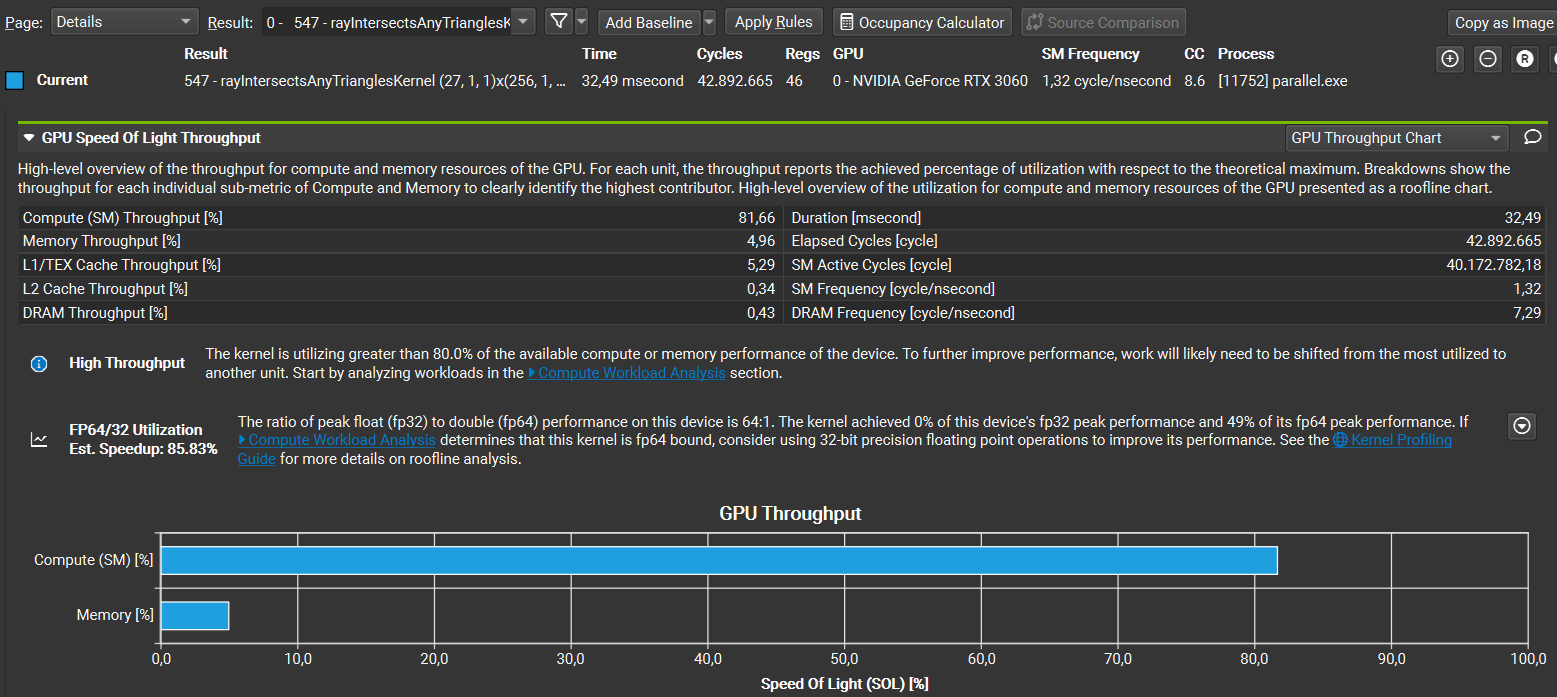
\includegraphics[width=0.98\textwidth]{images/parallel.png}
    \caption{Profiling per l'eseguibile parallelo senza SH}
\end{figure}

Analizzo poi il diagramma degli accessi in memoria, dai cui si nota come tutte le richieste passino dal Kernel, alla memoria globale (passando poi per le varie memorie cache) fino ad arrivare alla memoria del device.

\begin{figure}[ht]
    \centering
    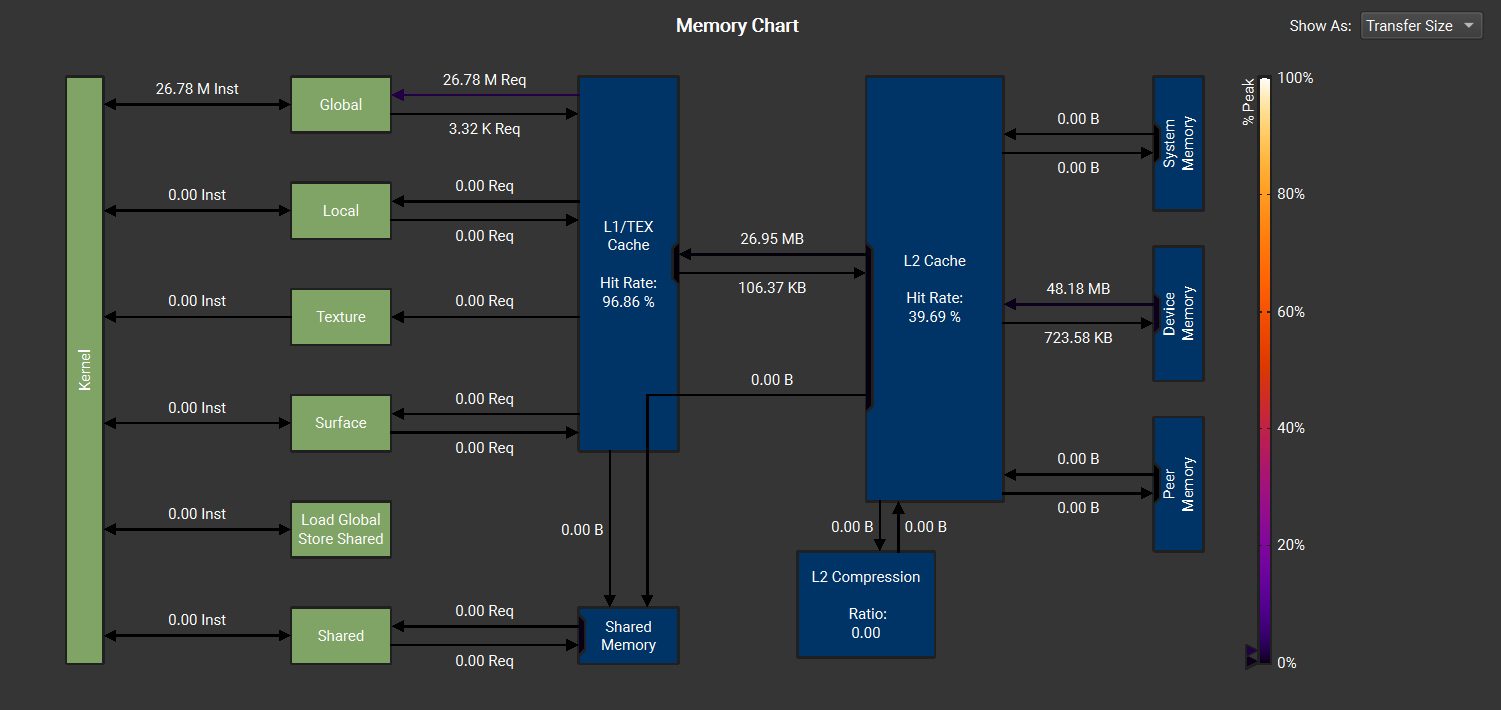
\includegraphics[width=0.98\textwidth]{images/parallel_chart.png}
    \caption{Memory access diagram per l'eseguibile parallelo senza SH}
\end{figure}


\subsubsection{Parallelo con SH (Size 256)}

Analizzando l'eseguibile che usa la shared memory, noto che anche in esso il tempo speso per la parte di computazione è quasi 15 volte superiore a quello per lo scambio dati in memoria (81.70\% contro il 4.99\%).

\begin{figure}[ht]
    \centering
    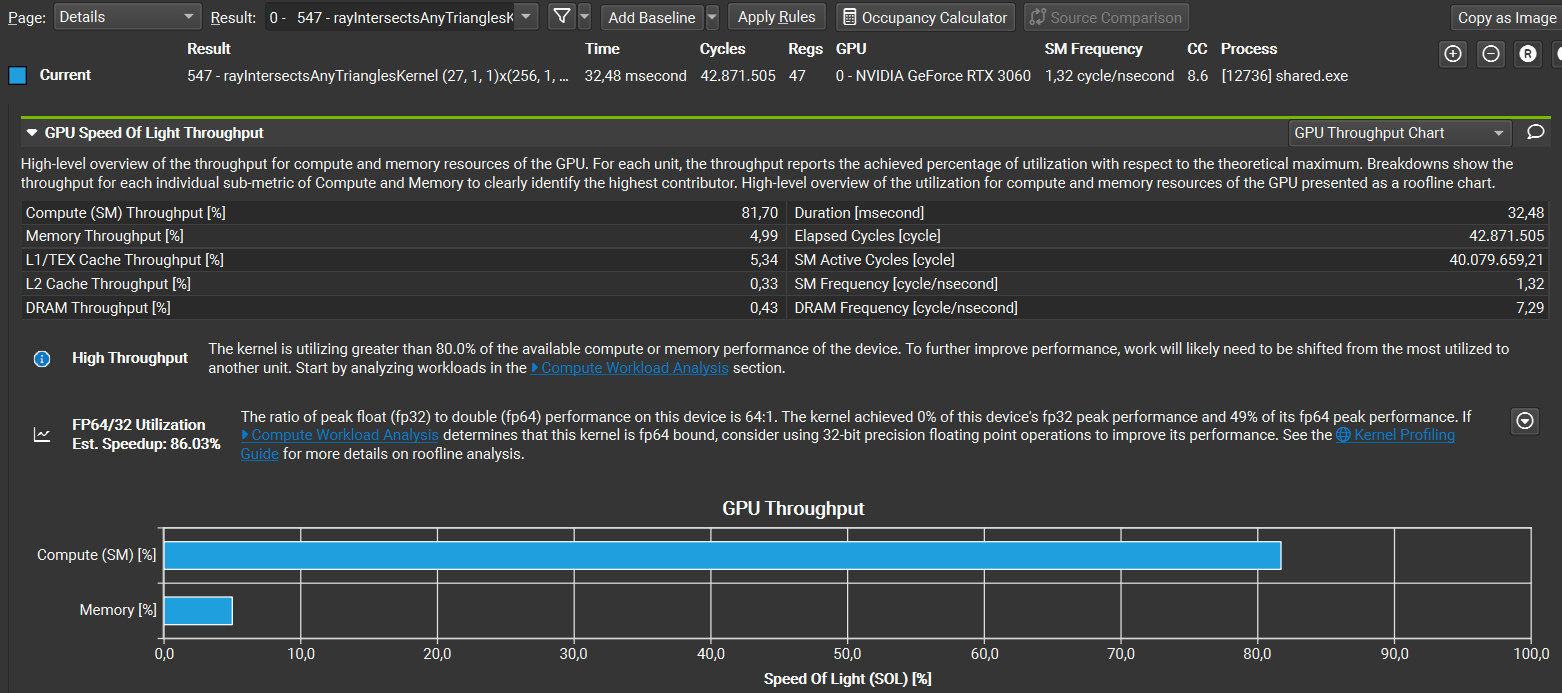
\includegraphics[width=0.98\textwidth]{images/shared.png}
    \caption{Profiling per l'eseguibile parallelo con SH}
\end{figure}

Invece, analizzando il diagramma degli accessi in memoria, si nota come quasi tutte le richieste passino dalla shared memory (passando poi per le varie memorie cache) fino ad arrivare alla memoria del device e questa è la motivazione delle prestazioni migliori.

\begin{figure}[ht]
    \centering
    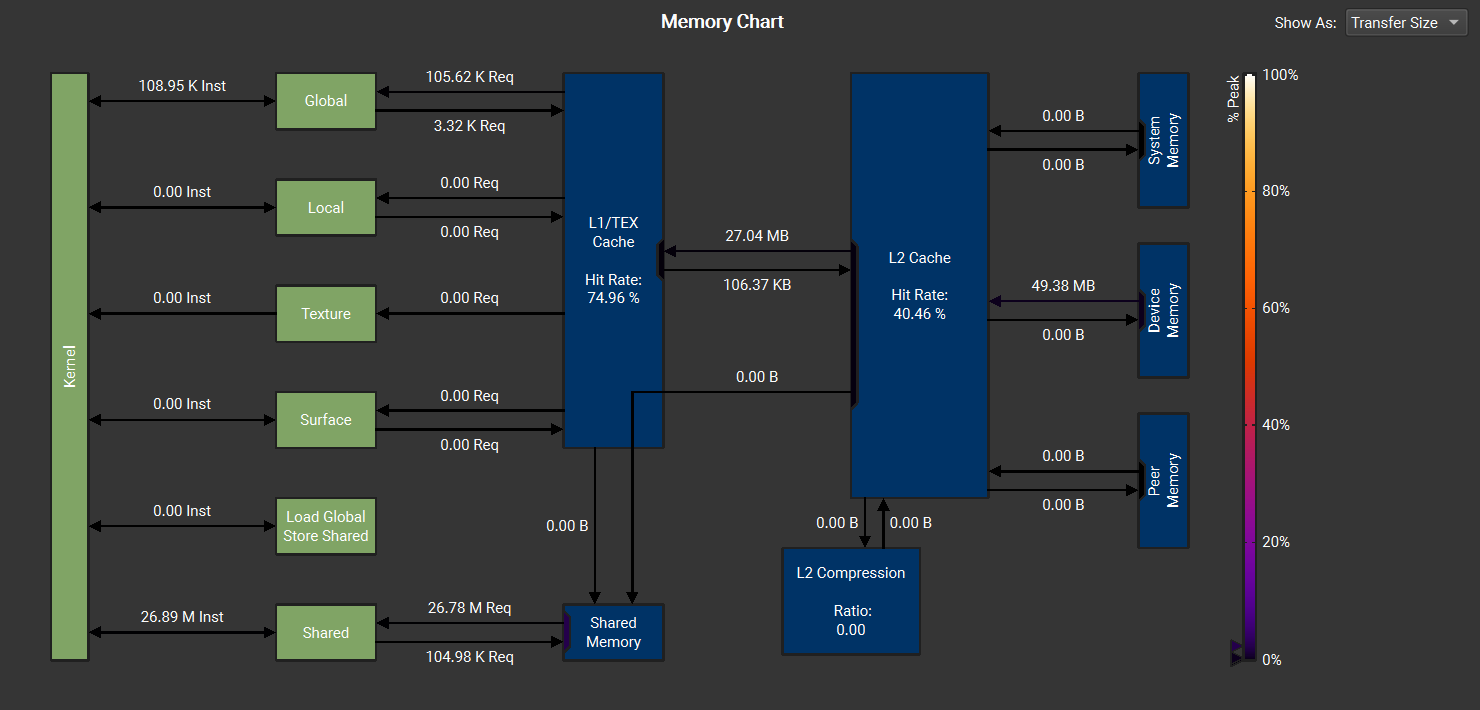
\includegraphics[width=0.98\textwidth]{images/shared_chart.png}
    \caption{Memory access diagram per l'eseguibile parallelo con SH}
\end{figure}

\subsection{Conclusioni}

Anche se siamo su un caso di studio abbastanza piccolo, l'esecuzione tramite CPU risulta essere circa 10 volte più lenta rispetto all'uso della GPU; inoltre implmentando la shared memory si vedono dei leggeri benefici, credo queste differenze verrebbero amplificate in un caso di studio più grande.

\end{document}